\section{Motivation \& Background}
\label{sec:motivation}
\loadFig{figPipeline}

\subsubsection{Modeling programs.} The problem of modeling source codes statistically has recently received academia's attention. The idea that programs can be treated as data-points in some high-dimensional space and using this representation to infer analysis tasks has seen modest success across different applications. These include predicting meaningful variable names \cite{}, presence of bugs and vulnerabilities \cite{}, grading programs \cite{}, etc. Each of these works models the problem as a supervised learning task, where features extracted from programs and are used to predict the property of interest. This is a seemingly lossy step, where the rich structural and semantic information present in programs is approximated via these features. A constant question which faces this community is choosing the right models which captures this rich information. Very recent work has explored using probabilistic graphical models, and graph neural networks to model problems inherently containing graph-like structures (e.g. synthesis of chemical compounds) \cite{}. This work is inspired by such an approach, and we lay out a strong argument for why this might be an appropriate modeling tool. We explore this on the problem of inferring variable types in programs.

\subsubsection{Inferring types.}
There exist deterministic algorithms like Hindley-Milner's W-algorithm (HM) to infer and check the types of variables in programs. HM assumes some known structure between how variables interact, and inductively applies type-propagation rules. This works well in practice for languages which have been designed keeping such analyses in mind. With languages like Javascript and Ruby though, implementing HM will result in poor specificity, with most types simply being inferred as \textit{any}. Such inference may not be very helpful to an end-user, and hence, warrants other techniques which may prove effective in discovering such information. 

We hence explore machine learning as a possible tool to help learn these types from. The key insight here is that the problem of inferring types involves two sub-tasks: one of finding a signal which can inform the type of a variable, and another of having a model of a structured network which can help accurately propagate this signal to other occurrences of the same variable, or variables that are similar to it.

\subsubsection{Graph neural networks.} 
Graph-structured input modalities to machine learning problems have been explored over the last decade in light of deep neural network architectures. Le Cun et al. published a position paper \cite{} which described learning on graph-structured input modalities as a convolutional neural network learning non-Euclidean filters. Deep Mind, with its recent position paper on inductive biases captured by graph neural networks \cite{}, has seemingly initiated a resurgence of interest in Graph neural networks (GNNs). 

Broadly, a popular architecture for a GNN is 

\loadFig{gnn}

It can be shown that this particular embedding of the program into the graph, along with the Graph Neural Network algorithm, roughly corresponds to performing posterior inference on a specific Markov Random Field that we believe approximates the true model of the type prediction problem.


\paragraph{Probabilistic interpretation.}
A Markov Random Field (MRF) is an undirected graphical model with the Markov assumption, that a node is conditionally independent from all other nodes given its neighbors~\cite{kinderman80markov}.
If we were to construct a Markov Random Field with an unobserved latent variable for each of our AST nodes, adding the various (undirected) edges described above, tag each node with an additional variable (the observed variable representing its AST type), and tag each variable with an additional variable representing its type, we would get a graph that looks roughly like Figure~\ref{fig:mrf-graph}.
We could then perform posterior inference on the type nodes of this graph using belief propagation~\cite{pearl2009causality}, which gives an approximate solution to the true posterior~\cite{weiss2000correctness}, giving our desired type predictions.
\begin{figure}
	\centering
	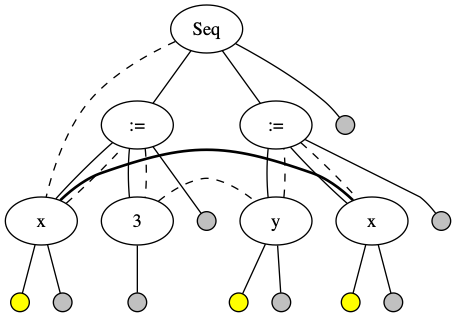
\includegraphics[width=\linewidth]{img/mrf_graph}
	\caption{Markov Random Field for an example program. Shaded nodes are observed, highlighted are posteriors}
	\label{fig:mrf-graph}
\end{figure}

We specifically argue the following two points:
\begin{enumerate*}[label=(\roman*)]
	\item the induced MRF is the correct model for this problem, and
	\item the graph neural network performs posterior inference on this network.
\end{enumerate*}

For point (i), we believe that the three classes of edges (AST edges, source file adjacency edges, and variable use edges) roughly capture the extent of conditional dependence in the model, in that the latent state of a variable (that predicts its type) is roughly conditionally independent from all others given its neighbors along those edges.
This is best argued through locality: the types of variables in a given region of code (e.g. inside of a function) are conditionally independent from the types of variables in a distance region of code (e.g. in a different function) given any variables that are shared or passed between them (the nonlocal \textsc{VariableUse} edges we add).
Some edges we added may be spurious, and while this may make it harder to perform inference (whether in the real MRF or our graph net), the MRF with too many edges can just be viewed as a refinement of the MRF with too few edges.
This is also the case with the undirectedness assumption, where it's likely that some of the edges would ideally be represented as directed edges.
However, this is also the case in using MRFs for images or other applications, and while the assumption can be shown to be at least somewhat incorrect there, MRFs still prove to be useful models~\cite{rangarajan95markov}.

Point (ii) requires arguing that our network architecture roughly performs posterior inference on the network.
This argument is much easier: belief propagation, a message passing algorithm, approximates the correct posterior on graphs with loops~\cite{weiss2000correctness}.
GNNs are in essence a message passing algorithm, where the messages are the result of some function learned by the GNN on the current latent state of a given node.
By merit of being neural networks, GNNs are capable of approximating any function~\cite{hornik1989multilayer} (and storing latent state), meaning that GNNs are capable of learning belief propagation (assuming we run the message passing for enough iterations).
Therefore, assuming that training our GNN finds its global optimum, we are guaranteed a solution at least as good as the approximate solution of belief propagation on the MRF, meaning that a GNN should be capable of solving the type inference problem.

\paragraph{Probabilistic interpretation.}
Having introduced the problem of type inference, and graph neural networks, we lay out a justification in this section for why such a network is the right form of inductive bias to be modeling programs.

A Markov Random Field (MRF) is an undirected graphical model with the Markov assumption, that a node is conditionally independent from all other nodes given its neighbors~\cite{kinderman80markov}.
If we were to construct a Markov Random Field with an unobserved latent variable for each of our AST nodes, adding the various (undirected) edges described above, tag each node with an additional variable (the observed variable representing its AST type), and tag each variable with an additional variable representing its type, we would get a graph that looks roughly like Figure~\ref{fig:mrf-graph}.
We could then perform posterior inference on the type nodes of this graph using belief propagation~\cite{pearl2009causality}, which gives an approximate solution to the true posterior~\cite{weiss2000correctness}, giving our desired type predictions.
\begin{figure}
	\centering
	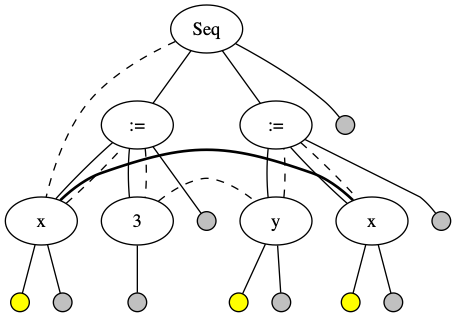
\includegraphics[width=\linewidth]{img/mrf_graph}
	\caption{Markov Random Field for an example program. Shaded nodes are observed, highlighted are posteriors}
	\label{fig:mrf-graph}
\end{figure}

We specifically argue the following two points:
\begin{enumerate*}[label=(\roman*)]
	\item the induced MRF is the correct model for this problem, and
	\item the graph neural network performs posterior inference on this network.
\end{enumerate*}

For point (i), we believe that the three classes of edges (AST edges, source file adjacency edges, and variable use edges) roughly capture the extent of conditional dependence in the model, in that the latent state of a variable (that predicts its type) is roughly conditionally independent from all others given its neighbors along those edges.
This is best argued through locality: the types of variables in a given region of code (e.g. inside of a function) are conditionally independent from the types of variables in a distance region of code (e.g. in a different function) given any variables that are shared or passed between them (the nonlocal \textsc{VariableUse} edges we add).
Some edges we added may be spurious, and while this may make it harder to perform inference (whether in the real MRF or our graph net), the MRF with too many edges can just be viewed as a refinement of the MRF with too few edges.
This is also the case with the undirectedness assumption, where it's likely that some of the edges would ideally be represented as directed edges.
However, this is also the case in using MRFs for images or other applications, and while the assumption can be shown to be at least somewhat incorrect there, MRFs still prove to be useful models~\cite{rangarajan95markov}.

Point (ii) requires arguing that our network architecture roughly performs posterior inference on the network.
This argument is much easier: belief propagation, a message passing algorithm, approximates the correct posterior on graphs with loops~\cite{weiss2000correctness}.
GNNs are in essence a message passing algorithm, where the messages are the result of some function learned by the GNN on the current latent state of a given node.
By merit of being neural networks, GNNs are capable of approximating any function~\cite{hornik1989multilayer} (and storing latent state), meaning that GNNs are capable of learning belief propagation (assuming we run the message passing for enough iterations).
Therefore, assuming that training our GNN finds its global optimum, we are guaranteed a solution at least as good as the approximate solution of belief propagation on the MRF, meaning that a GNN should be capable of solving the type inference problem.